% @Author: AnthonyKenny98
% @Date:   2020-04-08 09:52:59
% @Last Modified by:   AnthonyKenny98
% @Last Modified time: 2020-04-08 09:53:43
\subsection{Edge Collision Function}
\label{subsection:EdgeCollisionFunction}
    To briefly examine the edge collision detection function in general terms; Given an edge $e$, \gls{RRT} finds where $e$ intersects with grids in the \gls{OGM}. If any of the grids it intersects with are ``occupied'', a collision is returned. This is shown in Figure \ref{fig:edge_collision_process} on Page \pageref{fig:edge_collision_process}. 

    To see why it is so computationally intense to calculate intersections between a segment and grids, it must be understood that it is a fairly involved geometric process. Figure \ref{fig:edge_collision_planes} on Page \pageref{fig:edge_collision_planes} shows how grid intersections are detected by computing the where the segment intersects certain \textbf{\glspl{axis-oriented plane}}.  

    \subsubsection{Time Complexity}
        With the steps of the edge collision algorithm understood, (explained graphically in Figure \ref{fig:edge_collision_planes}, algorithm included in Appendix \ref{section:rrt_appendix_function_impl}, its \Gls{time complexity} may be quantified. 
        For an edge $e$ of maximum length $\epsilon$, it must check for intersections with $\epsilon \times \epsilon \times \epsilon$ grids. (i.e the only grids that are checked are the ones that the $e$ could possibly intersect with). 
        It first iterates through the three dimensions of \glspl{axis-oriented plane} ($xy$, $xz$, and $yz$). This is a constant of 3. 
        Within each of these dimensions, it must iterate through $\epsilon$ planes. This makes its time complexity $O(3\epsilon)$. 
        \todo{Appendix Reference?}% (Appendix C.[TODO] shows an $O(\epsilon^2)$ method upon which this is an improvement). 

        % @Author: AnthonyKenny98
% @Date:   2020-04-07 11:00:50
% @Last Modified by:   AnthonyKenny98
% @Last Modified time: 2020-04-07 12:40:47
\begin{figure}[H]
\begin{centering}
\begin{tabular}{cc}
    \begin{subfigure}{0.47\linewidth}
    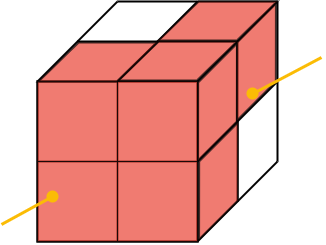
\includegraphics[width=\linewidth]{chapters/chapter3/img/edge_collision_planes_a.png}
    \caption{}
    \label{fig:edge_collision_planes_a}
    \end{subfigure} &

    \begin{subfigure}{0.47\linewidth}
    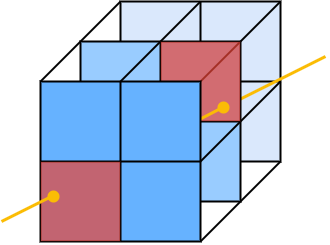
\includegraphics[width=\linewidth]{chapters/chapter3/img/edge_collision_planes_b.png}
    \caption{}
    \label{fig:edge_collision_planes_b}
    \end{subfigure} \\

    \begin{subfigure}{0.47\linewidth}
    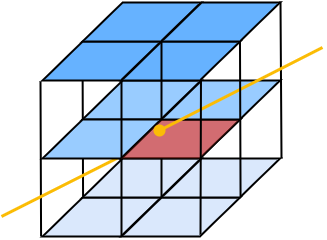
\includegraphics[width=\linewidth]{chapters/chapter3/img/edge_collision_planes_c.png}
    \caption{}
    \label{fig:edge_collision_planes_c}
    \end{subfigure} &

    \begin{subfigure}{0.47\linewidth}
    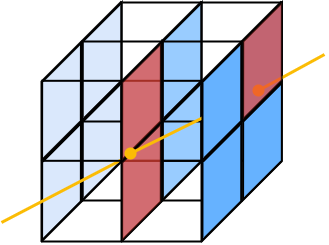
\includegraphics[width=\linewidth]{chapters/chapter3/img/edge_collision_planes_d.png}
    \caption{}
    \label{fig:edge_collision_planes_d}
    \end{subfigure} \\
\end{tabular}

\mycaption{Detecting Grid Intersections by Finding Intersections with Axis Oriented Planes}{\\ Consider an edge $e$ that spans the width of a $2\times 2\times 2$ grid map, as shown in Figure \ref{fig:edge_collision_planes} (do not consider if the grids are occupied, this is just to determine which of them the edge intersects). Just by eyeballing Figure \ref{fig:edge_collision_planes_a} it seems odd that so many of the grids have been intersected (denoted by red shading) by the yellow edge. The algorithm executed by checking one set of \glspl{axis-oriented plane} at a time. Figure \ref{fig:edge_collision_planes_a} shows how the $xy$-oriented planes are checked for 3 different values of $z$ (going into the page), finding two intersection points. There is only one intersection for the $xz$ oriented planes (\ref{fig:edge_collision_planes_c}). In Figure \ref{fig:edge_collision_planes_d}, the segment intersects 2 grids in the second $yz$-oriented plane, and one in the third plane. The intersected grids are thus any grid where a point-of-intersection falls on its face.}
\label{fig:edge_collision_planes}
\end{centering}
\end{figure}

        % @Author: AnthonyKenny98
% @Date:   2020-04-06 17:52:43
% @Last Modified by:   AnthonyKenny98
% @Last Modified time: 2020-04-06 17:52:43

   
\subsection{Technical Specifications}
\label{subsection:HoneyBeeSpecs}

    \subsubsection{Performance Specifications}
        When accelerating motion planning algorithms, it is often difficult to quantify a goal for how much faster one would like the function to run - the answer is usually ``as fast as possible!'' For this thesis, the performance specification was set to be the edge collision function to run fast enough such that it was no longer the bottleneck function. This translated to a desired speedup of about 3 times (when compared to benchmark performance of a typical CPU). Table \ref{table:edg_col_performance_specs} quantifies this in terms of latency and throughput.

        % @Author: AnthonyKenny98
% @Date:   2020-04-07 13:28:39
% @Last Modified by:   AnthonyKenny98
% @Last Modified time: 2020-04-08 16:26:52
\begin{table}[H]
\begin{centering}
\begin{tabular}{|c|c|c|}
\hline
\textbf{Metric}     &   \textbf{Benchmark CPU$^*$}   & \textbf{Accelerated} \\
\hline
Latency ($\mu$seconds/edge)  &   2.6  & 0.9 \\
\hline
Throughput (edges/second)  &   384,615  & 1,111,111 \\
\hline
\end{tabular}
\mycaption{Performance Specifications for Edge Collision Detection Unit}{. $^*$Benchmark CPU is an Intel 3.1 GHz i7 Dual Core processor, typical of a laptop computer.}
\label{table:edg_col_performance_specs}
\end{centering}
\end{table}

\newpage

\subsubsection{Area Specifications}
    Generally, an inverse relationship exists between latency and area. While it may be possible to make the unit much faster than the latency specification, this may become prohibitive with regards to the amount of area on chip it would occupy. It was decided to limit the area to that which would fit on an \gls{FPGA} typical in drone applications (those of the Kintex-7 Low Voltage family were chosen, but there are many possible options.) 

    Logic area on an FPGA is largely determined by \glspl{LUT}. \glsdesc{LUT_g} As such, the upper bound on area was set at 274,080 \glspl{LUT}.

    \subsubsection{Interface Specifications}
    \label{subsection:HoneyBeeTechSpechs}
        As shown in Figure \ref{fig:edge_collision_process}, the computationally intensive part of the process of edge collision detection is finding points of intersection between an edge and the grids of the map. Comparing this result to an \gls{OGM} is simple and fast. Therefore, it was decided that the hardware unit would simply take an edge and determine the grids with which it intersects. Whether the edge intersects a given grid can be represented as a binary $\{0,1\}$, and thus a the intersections found in a $\epsilon \times \epsilon\times\epsilon$ gridspace can be represented as an $\epsilon^3$ sequence of binary values.
        Table \ref{table:edg_col_interface_specs} outlines the required interface specifications for the functional unit.
        % @Author: AnthonyKenny98
% @Date:   2020-03-01 14:11:33
% @Last Modified by:   AnthonyKenny98
% @Last Modified time: 2020-04-07 14:09:51
\begin{table}[H]
\begin{center}
\begin{tabular}{|p{.2\linewidth}|p{.74\linewidth}|}
    \hline
    \textbf{Element}             & \textbf{Description/Justification} \\
    \hline
    \multicolumn{2}{|c|}{Constraints} \\
    \hline
    Length $\epsilon$  & $\epsilon$ defines the max edge length. The space being checked and the output sequence has the dimensions $\epsilon\times\epsilon\times\epsilon$ \\
    \hline
    \multicolumn{2}{|c|}{Inputs} \\
    \hline
    Edge $e$  & An Edge $e$ defined for a \gls{3D} \gls{configuration} space by two points $\{p1, p2\}$, each defined by a set of \gls{3D} coordinates $\{x,y,z\}$.\\
    \hline
    Control Inputs & The functional unit must have ports for control signals: clock, reset, start. These are required for adding the unit to a processor. \\
    \hline
    \multicolumn{2}{|c|}{Outputs} \\ 
    \hline
    Return Value & $\epsilon^3$ bit sequence: 1 if collides with grid at that index, 0 otherwise.\\
    \hline
    Control Outputs & Output ports for control signals: idle, done, ready. These are required for adding the unit to a processor. \\
    \hline
\end{tabular}
\mycaption{Interface Specifications for Edge Collision Detection Unit}{}
\label{table:edg_col_interface_specs}
\end{center}
\end{table}